% Created by tikzDevice version 0.10.1 on 2016-08-23 12:47:43
% !TEX encoding = UTF-8 Unicode
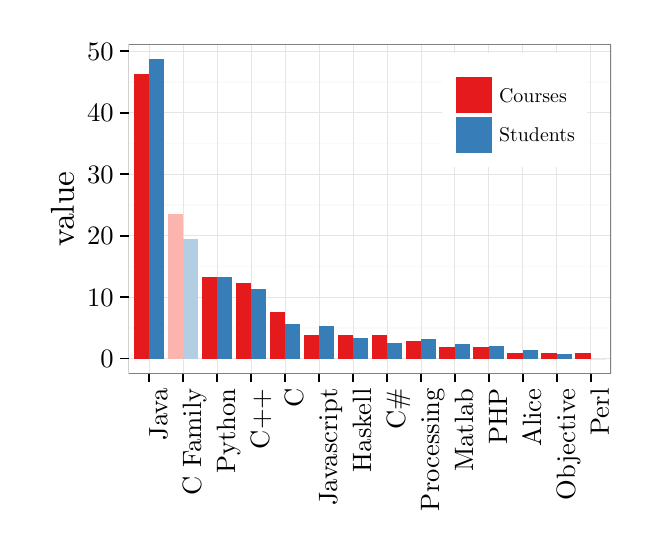
\begin{tikzpicture}[x=1pt,y=1pt]
\definecolor{fillColor}{RGB}{255,255,255}
\path[use as bounding box,fill=fillColor,fill opacity=0.00] (0,0) rectangle (216.81,180.67);
\begin{scope}
\path[clip] (  0.00,  0.00) rectangle (216.81,180.67);
\definecolor{drawColor}{RGB}{255,255,255}
\definecolor{fillColor}{RGB}{255,255,255}

\path[draw=drawColor,line width= 0.6pt,line join=round,line cap=round,fill=fillColor] (  0.00,  0.00) rectangle (216.81,180.68);
\end{scope}
\begin{scope}
\path[clip] ( 36.46, 55.66) rectangle (210.81,174.67);
\definecolor{fillColor}{RGB}{255,255,255}

\path[fill=fillColor] ( 36.46, 55.66) rectangle (210.81,174.68);
\definecolor{drawColor}{gray}{0.98}

\path[draw=drawColor,line width= 0.6pt,line join=round] ( 36.46, 72.18) --
	(210.81, 72.18);

\path[draw=drawColor,line width= 0.6pt,line join=round] ( 36.46, 94.40) --
	(210.81, 94.40);

\path[draw=drawColor,line width= 0.6pt,line join=round] ( 36.46,116.61) --
	(210.81,116.61);

\path[draw=drawColor,line width= 0.6pt,line join=round] ( 36.46,138.83) --
	(210.81,138.83);

\path[draw=drawColor,line width= 0.6pt,line join=round] ( 36.46,161.05) --
	(210.81,161.05);
\definecolor{drawColor}{gray}{0.90}

\path[draw=drawColor,line width= 0.2pt,line join=round] ( 36.46, 61.07) --
	(210.81, 61.07);

\path[draw=drawColor,line width= 0.2pt,line join=round] ( 36.46, 83.29) --
	(210.81, 83.29);

\path[draw=drawColor,line width= 0.2pt,line join=round] ( 36.46,105.50) --
	(210.81,105.50);

\path[draw=drawColor,line width= 0.2pt,line join=round] ( 36.46,127.72) --
	(210.81,127.72);

\path[draw=drawColor,line width= 0.2pt,line join=round] ( 36.46,149.94) --
	(210.81,149.94);

\path[draw=drawColor,line width= 0.2pt,line join=round] ( 36.46,172.16) --
	(210.81,172.16);

\path[draw=drawColor,line width= 0.2pt,line join=round] ( 43.83, 55.66) --
	( 43.83,174.67);

\path[draw=drawColor,line width= 0.2pt,line join=round] ( 56.11, 55.66) --
	( 56.11,174.67);

\path[draw=drawColor,line width= 0.2pt,line join=round] ( 68.39, 55.66) --
	( 68.39,174.67);

\path[draw=drawColor,line width= 0.2pt,line join=round] ( 80.66, 55.66) --
	( 80.66,174.67);

\path[draw=drawColor,line width= 0.2pt,line join=round] ( 92.94, 55.66) --
	( 92.94,174.67);

\path[draw=drawColor,line width= 0.2pt,line join=round] (105.22, 55.66) --
	(105.22,174.67);

\path[draw=drawColor,line width= 0.2pt,line join=round] (117.50, 55.66) --
	(117.50,174.67);

\path[draw=drawColor,line width= 0.2pt,line join=round] (129.78, 55.66) --
	(129.78,174.67);

\path[draw=drawColor,line width= 0.2pt,line join=round] (142.05, 55.66) --
	(142.05,174.67);

\path[draw=drawColor,line width= 0.2pt,line join=round] (154.33, 55.66) --
	(154.33,174.67);

\path[draw=drawColor,line width= 0.2pt,line join=round] (166.61, 55.66) --
	(166.61,174.67);

\path[draw=drawColor,line width= 0.2pt,line join=round] (178.89, 55.66) --
	(178.89,174.67);

\path[draw=drawColor,line width= 0.2pt,line join=round] (191.17, 55.66) --
	(191.17,174.67);

\path[draw=drawColor,line width= 0.2pt,line join=round] (203.44, 55.66) --
	(203.44,174.67);
\definecolor{fillColor}{RGB}{228,26,28}

\path[fill=fillColor] ( 38.30, 61.07) rectangle ( 43.83,163.78);
\definecolor{fillColor}{RGB}{55,126,184}

\path[fill=fillColor] ( 43.83, 61.07) rectangle ( 49.35,169.27);
\definecolor{fillColor}{RGB}{251,180,174}

\path[fill=fillColor] ( 50.58, 61.07) rectangle ( 56.11,113.47);
\definecolor{fillColor}{RGB}{179,205,227}

\path[fill=fillColor] ( 56.11, 61.07) rectangle ( 61.63,104.31);
\definecolor{fillColor}{RGB}{228,26,28}

\path[fill=fillColor] ( 62.86, 61.07) rectangle ( 68.39, 90.41);
\definecolor{fillColor}{RGB}{55,126,184}

\path[fill=fillColor] ( 68.39, 61.07) rectangle ( 73.91, 90.48);
\definecolor{fillColor}{RGB}{228,26,28}

\path[fill=fillColor] ( 75.14, 61.07) rectangle ( 80.66, 88.32);
\definecolor{fillColor}{RGB}{55,126,184}

\path[fill=fillColor] ( 80.66, 61.07) rectangle ( 86.19, 86.30);
\definecolor{fillColor}{RGB}{228,26,28}

\path[fill=fillColor] ( 87.42, 61.07) rectangle ( 92.94, 77.84);
\definecolor{fillColor}{RGB}{55,126,184}

\path[fill=fillColor] ( 92.94, 61.07) rectangle ( 98.47, 73.44);
\definecolor{fillColor}{RGB}{228,26,28}

\path[fill=fillColor] ( 99.69, 61.07) rectangle (105.22, 69.45);
\definecolor{fillColor}{RGB}{55,126,184}

\path[fill=fillColor] (105.22, 61.07) rectangle (110.74, 72.88);
\definecolor{fillColor}{RGB}{228,26,28}

\path[fill=fillColor] (111.97, 61.07) rectangle (117.50, 69.45);
\definecolor{fillColor}{RGB}{55,126,184}

\path[fill=fillColor] (117.50, 61.07) rectangle (123.02, 68.71);
\definecolor{fillColor}{RGB}{228,26,28}

\path[fill=fillColor] (124.25, 61.07) rectangle (129.78, 69.45);
\definecolor{fillColor}{RGB}{55,126,184}

\path[fill=fillColor] (129.78, 61.07) rectangle (135.30, 66.70);
\definecolor{fillColor}{RGB}{228,26,28}

\path[fill=fillColor] (136.53, 61.07) rectangle (142.05, 67.35);
\definecolor{fillColor}{RGB}{55,126,184}

\path[fill=fillColor] (142.05, 61.07) rectangle (147.58, 68.22);
\definecolor{fillColor}{RGB}{228,26,28}

\path[fill=fillColor] (148.81, 61.07) rectangle (154.33, 65.26);
\definecolor{fillColor}{RGB}{55,126,184}

\path[fill=fillColor] (154.33, 61.07) rectangle (159.86, 66.41);
\definecolor{fillColor}{RGB}{228,26,28}

\path[fill=fillColor] (161.08, 61.07) rectangle (166.61, 65.26);
\definecolor{fillColor}{RGB}{55,126,184}

\path[fill=fillColor] (166.61, 61.07) rectangle (172.13, 65.79);
\definecolor{fillColor}{RGB}{228,26,28}

\path[fill=fillColor] (173.36, 61.07) rectangle (178.89, 63.16);
\definecolor{fillColor}{RGB}{55,126,184}

\path[fill=fillColor] (178.89, 61.07) rectangle (184.41, 64.10);
\definecolor{fillColor}{RGB}{228,26,28}

\path[fill=fillColor] (185.64, 61.07) rectangle (191.17, 63.16);
\definecolor{fillColor}{RGB}{55,126,184}

\path[fill=fillColor] (191.17, 61.07) rectangle (196.69, 62.68);
\definecolor{fillColor}{RGB}{228,26,28}

\path[fill=fillColor] (197.92, 61.07) rectangle (203.44, 63.16);
\definecolor{fillColor}{RGB}{55,126,184}

\path[fill=fillColor] (203.44, 61.07) rectangle (208.97, 61.07);
\definecolor{drawColor}{gray}{0.50}

\path[draw=drawColor,line width= 0.6pt,line join=round,line cap=round] ( 36.46, 55.66) rectangle (210.81,174.68);
\end{scope}
\begin{scope}
\path[clip] (  0.00,  0.00) rectangle (216.81,180.67);
\definecolor{drawColor}{RGB}{0,0,0}

\node[text=drawColor,anchor=base east,inner sep=0pt, outer sep=0pt, scale=  0.96] at ( 31.06, 57.76) {0};

\node[text=drawColor,anchor=base east,inner sep=0pt, outer sep=0pt, scale=  0.96] at ( 31.06, 79.98) {10};

\node[text=drawColor,anchor=base east,inner sep=0pt, outer sep=0pt, scale=  0.96] at ( 31.06,102.20) {20};

\node[text=drawColor,anchor=base east,inner sep=0pt, outer sep=0pt, scale=  0.96] at ( 31.06,124.42) {30};

\node[text=drawColor,anchor=base east,inner sep=0pt, outer sep=0pt, scale=  0.96] at ( 31.06,146.64) {40};

\node[text=drawColor,anchor=base east,inner sep=0pt, outer sep=0pt, scale=  0.96] at ( 31.06,168.86) {50};
\end{scope}
\begin{scope}
\path[clip] (  0.00,  0.00) rectangle (216.81,180.67);
\definecolor{drawColor}{RGB}{0,0,0}

\path[draw=drawColor,line width= 0.6pt,line join=round] ( 33.46, 61.07) --
	( 36.46, 61.07);

\path[draw=drawColor,line width= 0.6pt,line join=round] ( 33.46, 83.29) --
	( 36.46, 83.29);

\path[draw=drawColor,line width= 0.6pt,line join=round] ( 33.46,105.50) --
	( 36.46,105.50);

\path[draw=drawColor,line width= 0.6pt,line join=round] ( 33.46,127.72) --
	( 36.46,127.72);

\path[draw=drawColor,line width= 0.6pt,line join=round] ( 33.46,149.94) --
	( 36.46,149.94);

\path[draw=drawColor,line width= 0.6pt,line join=round] ( 33.46,172.16) --
	( 36.46,172.16);
\end{scope}
\begin{scope}
\path[clip] (  0.00,  0.00) rectangle (216.81,180.67);
\definecolor{drawColor}{RGB}{0,0,0}

\path[draw=drawColor,line width= 0.6pt,line join=round] ( 43.83, 52.66) --
	( 43.83, 55.66);

\path[draw=drawColor,line width= 0.6pt,line join=round] ( 56.11, 52.66) --
	( 56.11, 55.66);

\path[draw=drawColor,line width= 0.6pt,line join=round] ( 68.39, 52.66) --
	( 68.39, 55.66);

\path[draw=drawColor,line width= 0.6pt,line join=round] ( 80.66, 52.66) --
	( 80.66, 55.66);

\path[draw=drawColor,line width= 0.6pt,line join=round] ( 92.94, 52.66) --
	( 92.94, 55.66);

\path[draw=drawColor,line width= 0.6pt,line join=round] (105.22, 52.66) --
	(105.22, 55.66);

\path[draw=drawColor,line width= 0.6pt,line join=round] (117.50, 52.66) --
	(117.50, 55.66);

\path[draw=drawColor,line width= 0.6pt,line join=round] (129.78, 52.66) --
	(129.78, 55.66);

\path[draw=drawColor,line width= 0.6pt,line join=round] (142.05, 52.66) --
	(142.05, 55.66);

\path[draw=drawColor,line width= 0.6pt,line join=round] (154.33, 52.66) --
	(154.33, 55.66);

\path[draw=drawColor,line width= 0.6pt,line join=round] (166.61, 52.66) --
	(166.61, 55.66);

\path[draw=drawColor,line width= 0.6pt,line join=round] (178.89, 52.66) --
	(178.89, 55.66);

\path[draw=drawColor,line width= 0.6pt,line join=round] (191.17, 52.66) --
	(191.17, 55.66);

\path[draw=drawColor,line width= 0.6pt,line join=round] (203.44, 52.66) --
	(203.44, 55.66);
\end{scope}
\begin{scope}
\path[clip] (  0.00,  0.00) rectangle (216.81,180.67);
\definecolor{drawColor}{RGB}{0,0,0}

\node[text=drawColor,rotate= 90.00,anchor=base east,inner sep=0pt, outer sep=0pt, scale=  0.96] at ( 50.44, 50.26) {Java};

\node[text=drawColor,rotate= 90.00,anchor=base east,inner sep=0pt, outer sep=0pt, scale=  0.96] at ( 62.72, 50.26) {C Family};

\node[text=drawColor,rotate= 90.00,anchor=base east,inner sep=0pt, outer sep=0pt, scale=  0.96] at ( 75.00, 50.26) {Python};

\node[text=drawColor,rotate= 90.00,anchor=base east,inner sep=0pt, outer sep=0pt, scale=  0.96] at ( 87.27, 50.26) {C++};

\node[text=drawColor,rotate= 90.00,anchor=base east,inner sep=0pt, outer sep=0pt, scale=  0.96] at ( 99.55, 50.26) {C};

\node[text=drawColor,rotate= 90.00,anchor=base east,inner sep=0pt, outer sep=0pt, scale=  0.96] at (111.83, 50.26) {Javascript};

\node[text=drawColor,rotate= 90.00,anchor=base east,inner sep=0pt, outer sep=0pt, scale=  0.96] at (124.11, 50.26) {Haskell};

\node[text=drawColor,rotate= 90.00,anchor=base east,inner sep=0pt, outer sep=0pt, scale=  0.96] at (136.39, 50.26) {C\#};

\node[text=drawColor,rotate= 90.00,anchor=base east,inner sep=0pt, outer sep=0pt, scale=  0.96] at (148.66, 50.26) {Processing};

\node[text=drawColor,rotate= 90.00,anchor=base east,inner sep=0pt, outer sep=0pt, scale=  0.96] at (160.94, 50.26) {Matlab};

\node[text=drawColor,rotate= 90.00,anchor=base east,inner sep=0pt, outer sep=0pt, scale=  0.96] at (173.22, 50.26) {PHP};

\node[text=drawColor,rotate= 90.00,anchor=base east,inner sep=0pt, outer sep=0pt, scale=  0.96] at (185.50, 50.26) {Alice};

\node[text=drawColor,rotate= 90.00,anchor=base east,inner sep=0pt, outer sep=0pt, scale=  0.96] at (197.78, 50.26) {Objective};

\node[text=drawColor,rotate= 90.00,anchor=base east,inner sep=0pt, outer sep=0pt, scale=  0.96] at (210.05, 50.26) {Perl};
\end{scope}
\begin{scope}
\path[clip] (  0.00,  0.00) rectangle (216.81,180.67);
\definecolor{drawColor}{RGB}{0,0,0}

\node[text=drawColor,rotate= 90.00,anchor=base,inner sep=0pt, outer sep=0pt, scale=  1.20] at ( 16.66,115.17) {value};
\end{scope}
\begin{scope}
\path[clip] (  0.00,  0.00) rectangle (216.81,180.67);
\definecolor{fillColor}{RGB}{255,255,255}

\path[fill=fillColor] (149.83,130.34) rectangle (202.06,171.40);
\end{scope}
\begin{scope}
\path[clip] (  0.00,  0.00) rectangle (216.81,180.67);
\definecolor{fillColor}{RGB}{228,26,28}

\path[fill=fillColor] (154.80,149.78) rectangle (167.84,162.81);
\end{scope}
\begin{scope}
\path[clip] (  0.00,  0.00) rectangle (216.81,180.67);
\definecolor{fillColor}{RGB}{55,126,184}

\path[fill=fillColor] (154.80,135.32) rectangle (167.84,148.35);
\end{scope}
\begin{scope}
\path[clip] (  0.00,  0.00) rectangle (216.81,180.67);
\definecolor{drawColor}{RGB}{0,0,0}

\node[text=drawColor,anchor=base west,inner sep=0pt, outer sep=0pt, scale=  0.72] at (170.35,153.81) {Courses};
\end{scope}
\begin{scope}
\path[clip] (  0.00,  0.00) rectangle (216.81,180.67);
\definecolor{drawColor}{RGB}{0,0,0}

\node[text=drawColor,anchor=base west,inner sep=0pt, outer sep=0pt, scale=  0.72] at (170.35,139.36) {Students};
\end{scope}
\end{tikzpicture}
